% !TeX root = ../../main.tex

\section{Introducción}
Data Analytics y Data Analysis son conceptos relacionados con el uso de los
datos. Aunque en algunas ocasiones se utilizan como sinónimos, tienen un
alcance diferente. Data Analytics comprende un proceso amplio que busca
convertir los datos en información útil para tomar decisiones. Por su parte,
Data Analysis se concentra en examinar datos específicos para encontrar
patrones, explicar resultados y obtener conclusiones.

\section{Data Analytics}
Data Analytics es una disciplina que utiliza datos, herramientas tecnológicas
y métodos estadísticos para generar información útil. Su propósito es ayudar
a las organizaciones a tomar mejores decisiones, detectar oportunidades,
identificar riesgos y anticipar posibles resultados.

Este concepto abarca varias etapas, como la recopilación, organización,
limpieza, análisis y presentación de los datos. También puede emplear modelos
predictivos para estimar lo que podría ocurrir en el futuro.

\subsection{características principales}

\begin{itemize}
    \item Tiene un alcance amplio.
    \item Puede trabajar con distintas fuentes de datos.
    \item Ayuda a detectar tendencias y oportunidades.
    \item Permite realizar predicciones.
    \item Apoya la toma de decisiones.
    \item Produce tableros, modelos y recomendaciones.
\end{itemize}

\subsection{Ejemplo}
Una tienda puede utilizar Data Analytics para estudiar sus ventas anteriores,
predecir la demanda de los siguientes meses y decidir cuánto inventario debe
comprar.

\subsection{Mapa mental Data Analytics}
\begin{figure}[H]
    \centering
    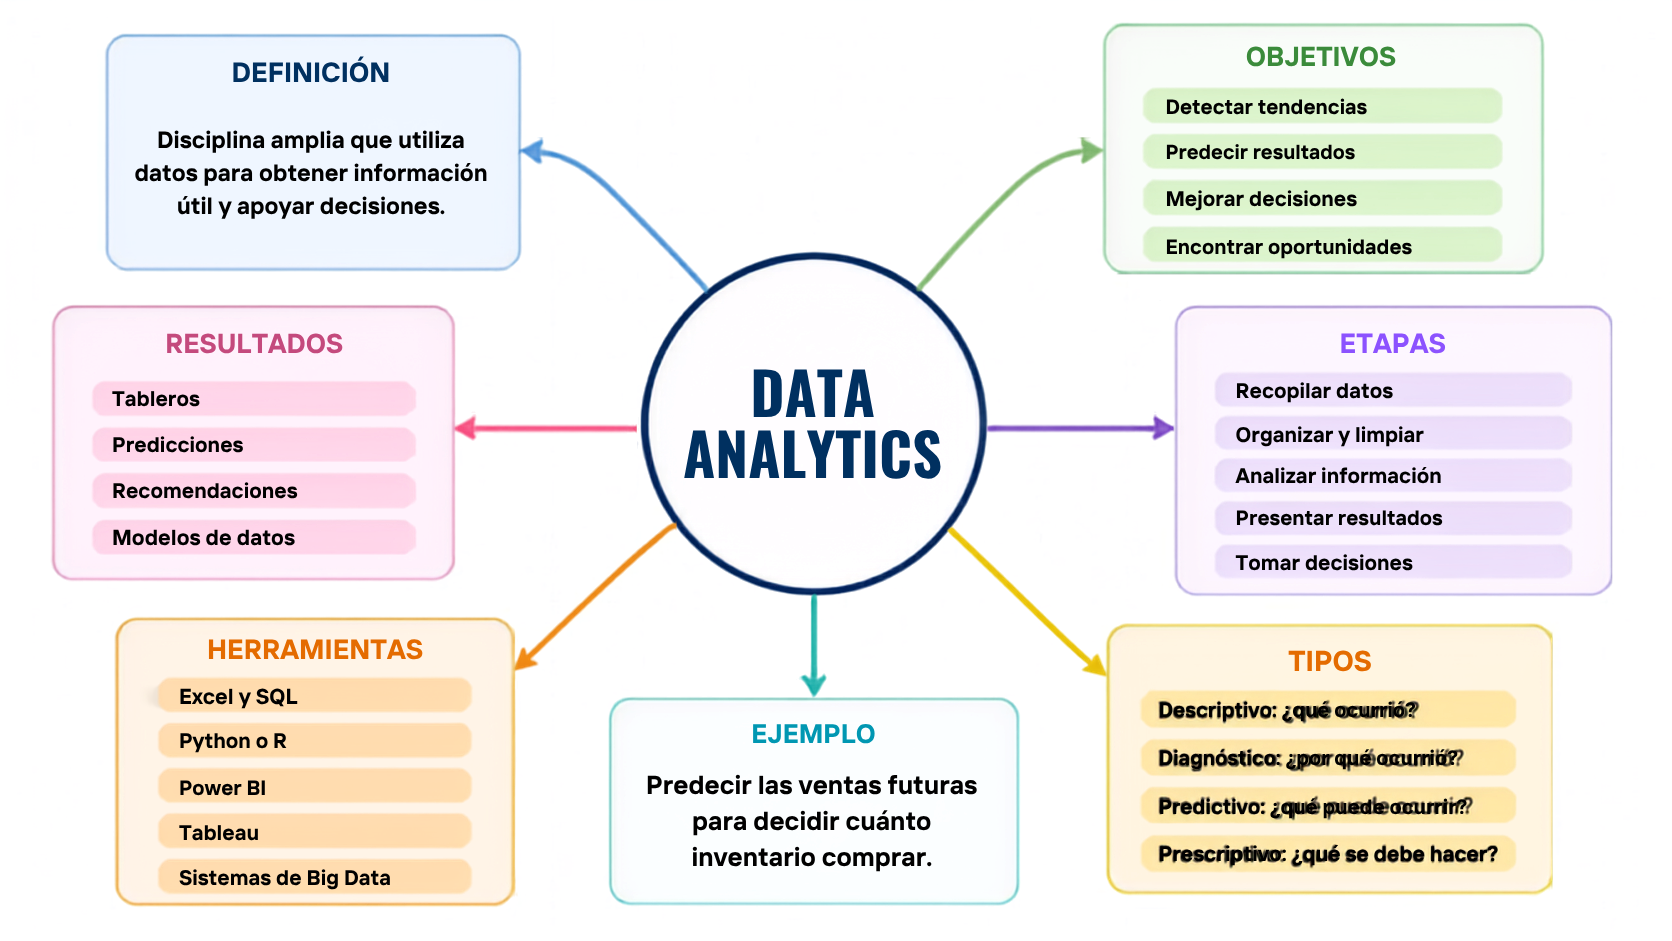
\includegraphics[width=0.90\textwidth]{actividades/1.26-actividad-7/img/data-analytics.png}
    \caption{Mapa mental Data Analytics}
    \label{fig:mapa-data-analytics}
\end{figure}

\section{Data Analysis}
Data Analysis es el proceso de examinar, limpiar, organizar e interpretar un
conjunto de datos. Su objetivo es descubrir información importante, responder
una pregunta específica y obtener conclusiones basadas en los resultados.

Este proceso puede incluir el uso de tablas, gráficas, promedios, porcentajes
y comparaciones. Generalmente se enfoca en comprender qué ocurrió y cuáles
fueron las posibles causas.

\subsection{Características principales}

\begin{itemize}
    \item Se concentra en un problema específico.
    \item Examina uno o varios conjuntos de datos definidos.
    \item Permite encontrar patrones y relaciones.
    \item Ayuda a comprender resultados anteriores.
    \item Utiliza tablas, gráficas y medidas estadísticas.
    \item Produce hallazgos, informes y conclusiones.
\end{itemize}

\subsection{Ejemplo}

Una empresa puede realizar un análisis de sus ventas mensuales para identificar
qué productos se vendieron más y en qué meses disminuyeron sus ingresos.

\subsection{Mapa mental de Data Analysis}
\begin{figure}[H]
    \centering
    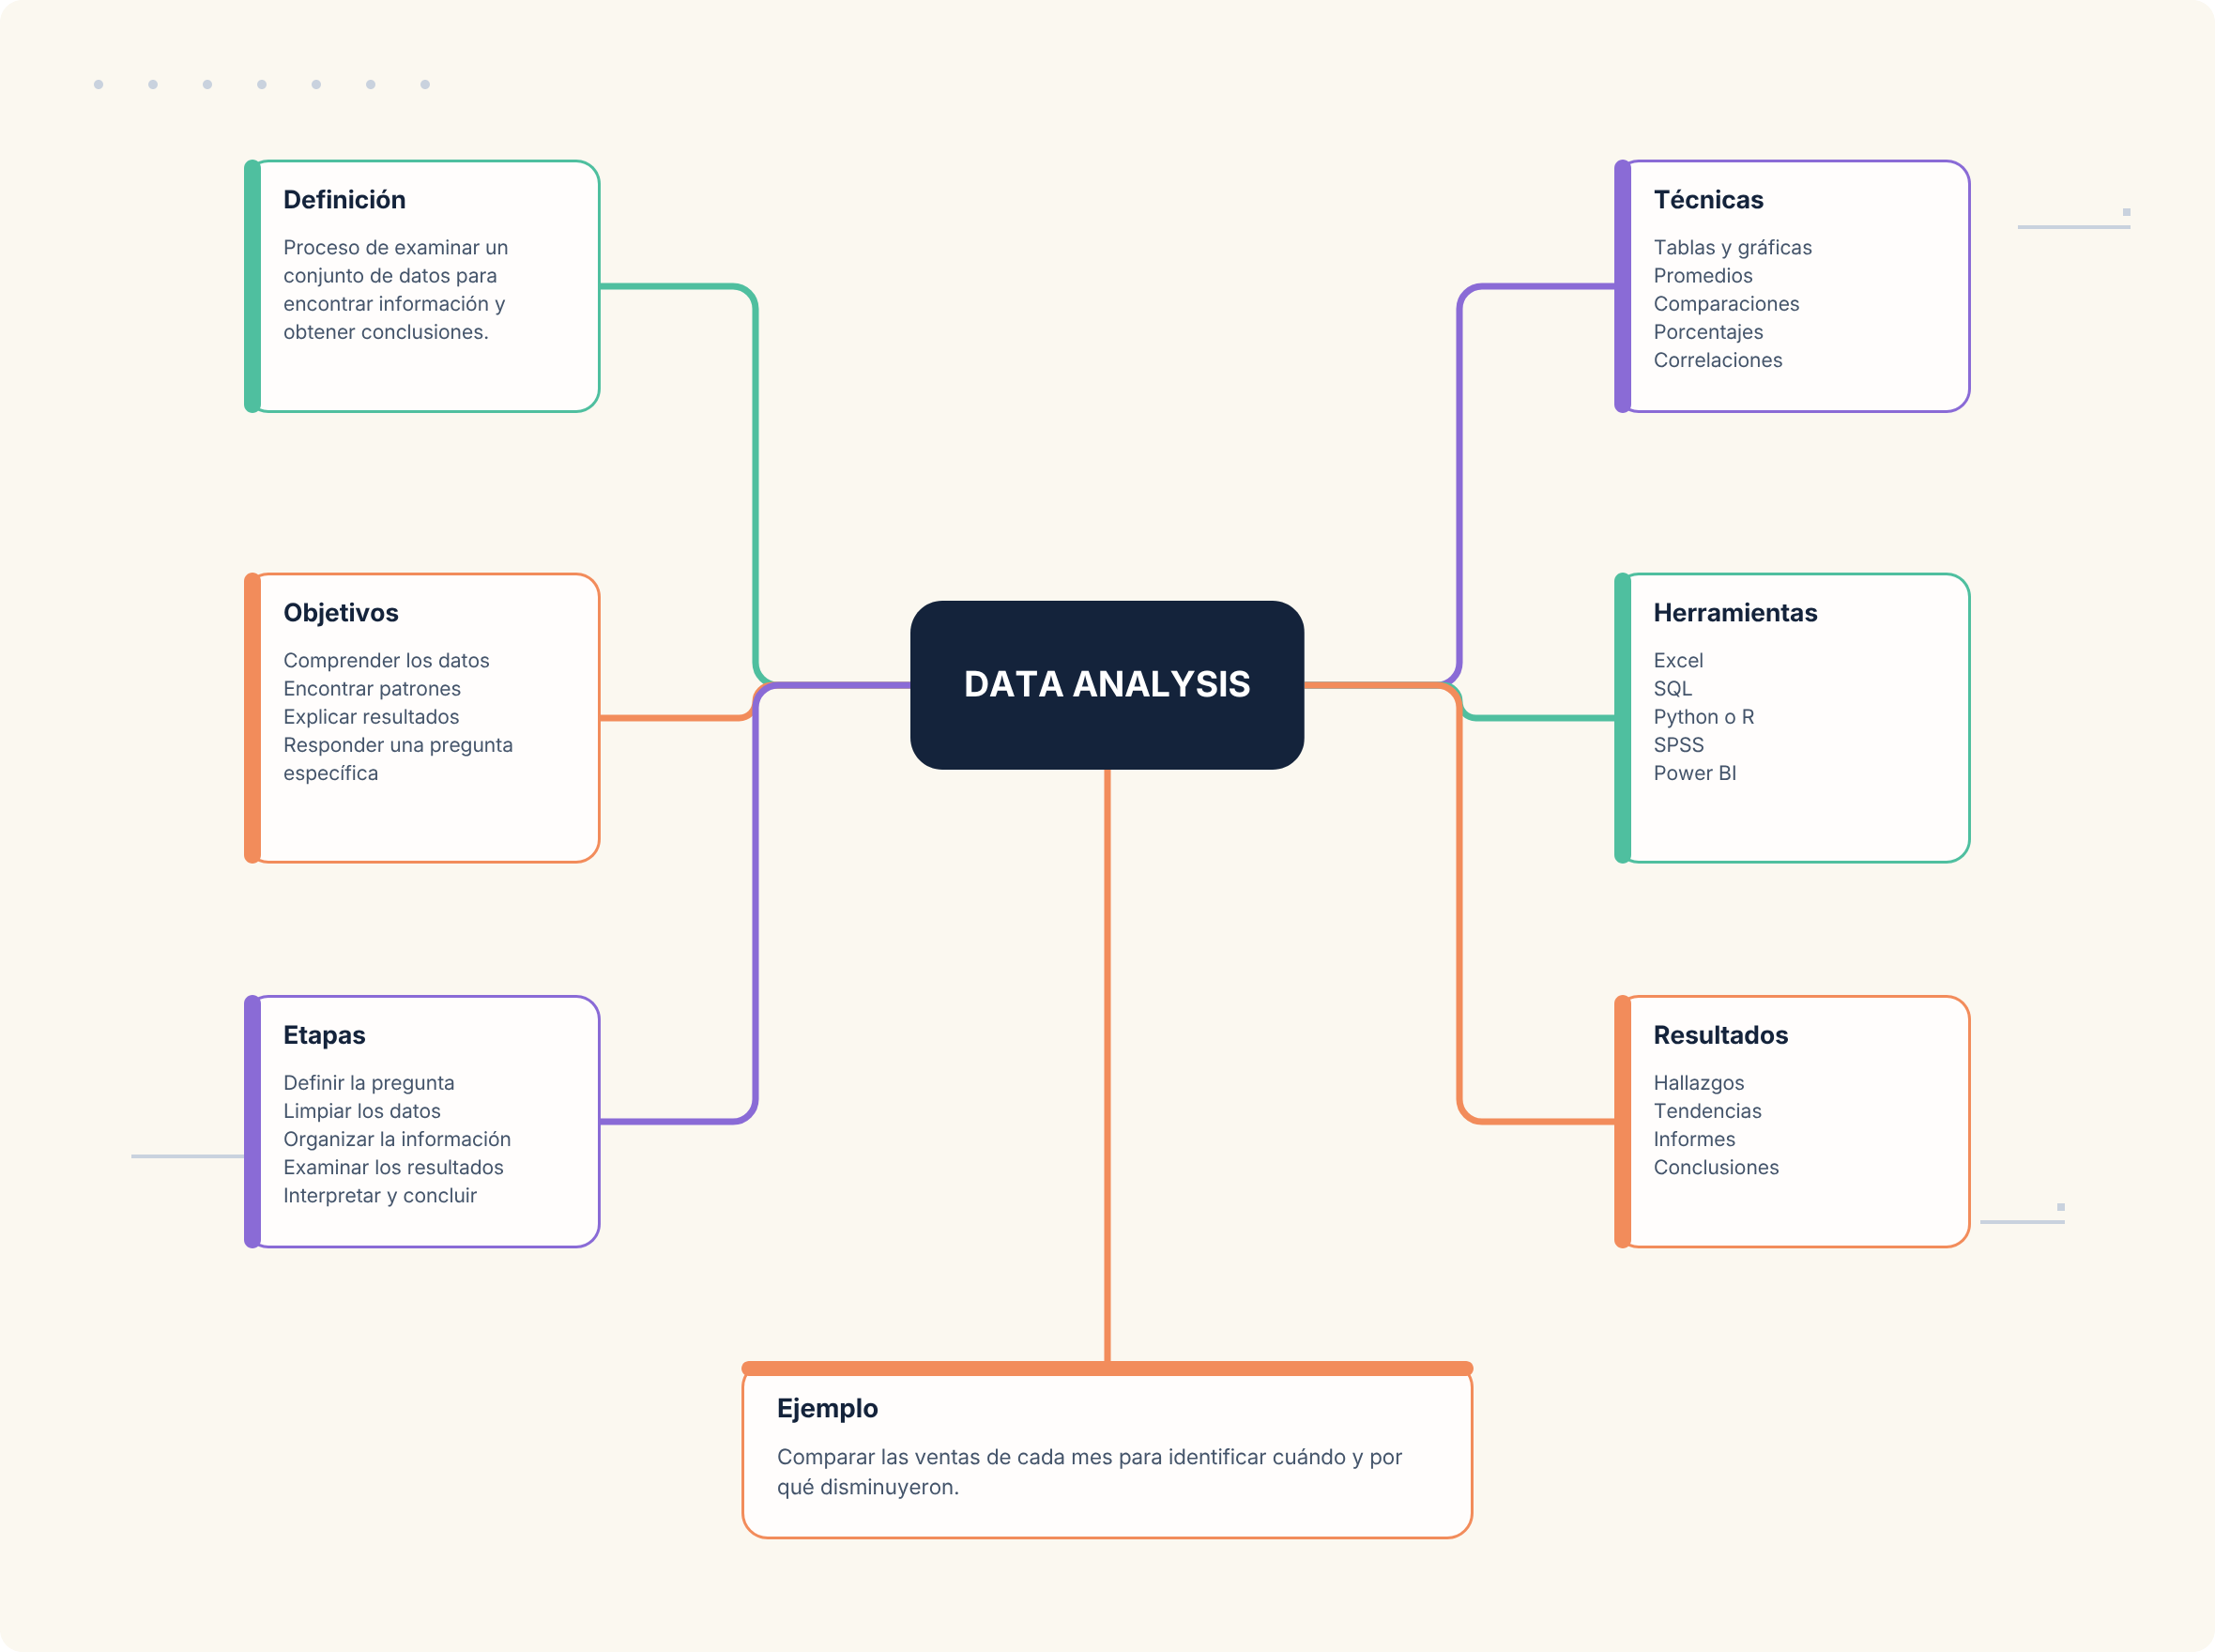
\includegraphics[width=0.90\textwidth]{actividades/1.26-actividad-7/img/data-analysis.png}
    \caption{Mapa mental data Analysis}
    \label{fig:mapa-data-analysis}
\end{figure}

\section{Comparación}

\begin{table}[H]
    \centering
    \caption{Comparación entre Data Analytics vs Data Analysis}
    \label{tab:comparacion}
    \renewcommand{\arraystretch}{1.4}
    \small

    \begin{tabularx}{\textwidth}{|p{3cm}|X|X|}
        \hline
        \textbf{Aspecto} &
        \textbf{Data Analytics} &
        \textbf{Data Analysis} \\
        \hline

        Alcance &
        Es una disciplina amplia que contiene diferentes etapas del trabajo con datos. &
        Es una actividad específica dentro del proceso analítico. \\
        \hline

        Objetivo &
        Apoyar decisiones y anticipar posibles resultados. &
        Examinar datos para encontrar información y obtener conclusiones. \\
        \hline

        Preguntas principales &
        ¿Qué puede ocurrir? ¿Qué decisión se debe tomar? &
        ¿Qué ocurrió? ¿Por qué ocurrió? \\
        \hline

        Orientación &
        Puede enfocarse en el presente y en el futuro. &
        Generalmente estudia datos históricos o actuales. \\
        \hline

        Actividades &
        Recopilar, integrar, analizar, modelar y comunicar datos. &
        Limpiar, organizar, examinar e interpretar datos. \\
        \hline

        Resultados &
        Predicciones, tableros, modelos y recomendaciones. &
        Hallazgos, tendencias, gráficas e informes. \\
        \hline

        Ejemplo &
        Predecir las ventas y recomendar una cantidad de inventario. &
        Comparar las ventas mensuales para detectar una disminución. \\
        \hline     
    \end{tabularx}
\end{table}

\section{Conclusión}
Data Analytics y Data Analysis son actividades complementarias. Data Analysis
permite comprender la información disponible y obtener conclusiones sobre una
situación específica. Data Analytics utiliza estos resultados junto con otras
herramientas y procesos para apoyar decisiones y anticipar escenarios futuros.
Por esta razón, ambos conceptos son importantes para aprovechar los datos de
manera adecuada.